% Chapter 20, Section 2

\section{Generative Adversarial Networks (GANs) \difficultyInline{advanced}}
\label{sec:gans}

GANs train two competing neural networks—a generator that creates fake data and a discriminator that tries to detect the fakes—in an adversarial game that eventually produces highly realistic synthetic samples.

\subsection{Core Idea}

The fundamental concept behind GANs is elegantly simple yet powerful. Imagine an art forger trying to create paintings so convincing that even expert art critics cannot distinguish them from genuine masterpieces. The forger (generator) continuously improves their technique based on feedback from the critics (discriminator), while the critics become more sophisticated at detecting fakes. This adversarial relationship drives both parties to become increasingly skilled—the forger learns to create more realistic art, while the critics develop sharper detection abilities.

In the GAN framework, the generator $G$ takes random noise as input and transforms it into synthetic data samples that should be indistinguishable from real data. The discriminator $D$ acts as a binary classifier, receiving both real and generated samples and learning to distinguish between them. As training progresses, the generator becomes increasingly adept at fooling the discriminator, while the discriminator becomes better at detecting subtle differences between real and fake samples.

\begin{figure}[h]
  \centering
  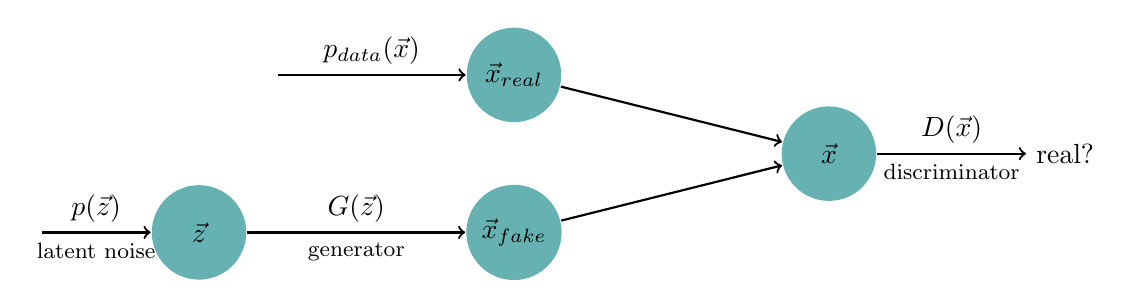
\begin{tikzpicture}[
    ->, thick,
    node/.style={circle, fill=teal!60, minimum size=1.2cm},
    label/.style={below, font=\footnotesize},
  ]

  % Generator path
  \node[node] (zin) at (0,0) {$\vec z$};
  \node[node] (fake) at (4,0) {$\vec x_\text{fake}$};
  \draw (zin) -- node[above] {$G(\vec z)$} node[label] {generator} (fake);

  % Real data path
  \node[node] (real) at (4,2) {$\vec x_\text{real}$};
  \draw[<-] (real) -- node[above] {$p_\text{data}(\vec x)$} ++(-3,0);

  % Discriminator
  \node[node] (D) at (8,1) {$\vec x$};
  \node (out) at (11,1) {real?};
  \draw (D) -- node[above] {$D(\vec x)$} node[label] {discriminator} (out);

  % Connections to discriminator
  \draw (fake) -- (D);
  \draw (real) -- (D);

  % Noise source
  \draw[<-] (zin) -- node[above] {$p(\vec z)$} node[label] {latent noise} ++(-2,0);

\end{tikzpicture}
\caption{GAN architecture showing the adversarial relationship between generator and discriminator.}
\label{fig:gan-architecture}
\end{figure}

\subsection{Objective}

Minimax game:
\begin{equation}
\min_G \max_D \mathbb{E}_{\vect{x} \sim p_{\text{data}}}[\log D(\vect{x})] + \mathbb{E}_{\vect{z} \sim p(\vect{z})}[\log(1 - D(G(\vect{z})))]
\end{equation}

The GAN objective represents a minimax game where the discriminator aims to maximize its ability to distinguish real from fake samples, while the generator seeks to minimize the discriminator's accuracy. The first term $\mathbb{E}_{\vect{x} \sim p_{\text{data}}}[\log D(\vect{x})]$ encourages the discriminator to assign high probability to real samples, while the second term $\mathbb{E}_{\vect{z} \sim p(\vect{z})}[\log(1 - D(G(\vect{z})))]$ penalizes the discriminator for correctly identifying generated samples, simultaneously training the generator to produce more convincing fakes.

\subsection{Training Procedure}

The training process alternates between updating the discriminator and generator in a carefully orchestrated dance. During each training iteration, the discriminator is first updated to improve its ability to distinguish real from fake samples. This involves maximizing the objective $\max_D \mathbb{E}_{\vect{x}}[\log D(\vect{x})] + \mathbb{E}_{\vect{z}}[\log(1 - D(G(\vect{z})))]$, which simultaneously rewards correct identification of real samples and penalizes misclassification of generated samples.

Following the discriminator update, the generator is trained to produce samples that are more likely to fool the updated discriminator. The generator's objective $\min_G \mathbb{E}_{\vect{z}}[\log(1 - D(G(\vect{z})))]$ encourages it to generate samples that the discriminator will classify as real. This alternating optimization process continues until the generator produces samples that are indistinguishable from real data, at which point the discriminator can no longer provide meaningful gradients for further improvement.

\subsection{Training Challenges}

GAN training presents several formidable challenges that can derail the delicate balance between generator and discriminator. Mode collapse occurs when the generator discovers a small subset of samples that consistently fool the discriminator, causing it to generate only these limited variations rather than exploring the full diversity of the data distribution. This phenomenon is particularly problematic when the discriminator becomes too strong relative to the generator, creating a feedback loop where the generator finds it easier to repeatedly generate the same convincing samples rather than learning the full data manifold.

Training instability manifests as oscillatory behavior where the generator and discriminator continuously outmaneuver each other without reaching a stable equilibrium. The discriminator may become too powerful, providing vanishing gradients to the generator, or the generator may become too skilled, causing the discriminator to lose its ability to provide meaningful learning signals. This instability often leads to non-convergence, where the training process fails to reach a meaningful solution despite extensive optimization efforts.

\subsection{GAN Variants}

The evolution of GAN architectures has addressed many of the fundamental challenges in adversarial training through innovative design choices and theoretical insights. DCGAN introduced architectural guidelines that stabilized training by using strided convolutions, batch normalization, and ReLU activations, establishing a foundation for successful deep convolutional GANs. WGAN revolutionized the field by replacing the Jensen-Shannon divergence with the Wasserstein distance, providing more stable gradients and better convergence properties that significantly reduced training instability.

StyleGAN represents a breakthrough in high-quality image generation by introducing a style-based generator architecture that separates high-level attributes from stochastic variation, enabling fine-grained control over generated images. Conditional GANs extend the basic framework by incorporating auxiliary information such as class labels, allowing for controlled generation of specific types of content. CycleGAN addresses the challenge of unpaired image-to-image translation by introducing cycle consistency constraints, enabling style transfer between domains without requiring paired training data.

% \subsection{Visual aids}
% \addcontentsline{toc}{subsubsection}{Visual aids (GANs)}

% \begin{figure}[h]
%   \centering
%   \begin{tikzpicture}[>=stealth]
%     \tikzstyle{b}=[draw,rounded corners,align=center,minimum width=2.4cm,minimum height=1.0cm]
%     \node[b,fill=bookpurple!10] at (0,0) (z) {Noise $\vect{z}$};
%     \node[b,fill=bookpurple!15] at (3.2,0) (g) {Generator $G$};
%     \node[b,fill=bookpurple!10] at (6.4,0.9) (x) {Real $\vect{x}$};
%     \node[b,fill=bookpurple!10] at (6.4,-0.9) (gx) {$G(\vect{z})$};
%     \node[b,fill=bookpurple!20] at (9.6,0) (d) {Discriminator $D$};
%     \draw[->] (z) -- (g);
%     \draw[->] (g) -- (gx);
%     \draw[->] (x) -- (d);
%     \draw[->] (gx) -- (d);
%   \end{tikzpicture}
%   \caption{GAN training: generator produces samples to fool discriminator.}
%   \label{fig:gan-diagram}
% \end{figure}

% \subsection{Notes and references}

% See \textcite{Goodfellow2014,GoodfellowEtAl2016,Prince2023} for GAN fundamentals and variants.

